\documentclass[aspectratio=169]{beamer}

% Theme selection
\usetheme{Madrid}
\usecolortheme{default}

% Packages
\usepackage[utf8]{inputenc}
\usepackage[T1]{fontenc}
\usepackage{graphicx}
\usepackage{booktabs}
\usepackage{hyperref}
\usepackage{tikz}
\usepackage{listings}
\usetikzlibrary{shapes,arrows,shadows,positioning,calc}

% Metadata
\title[Lightweight Semantic Structuring]{Lightweight Semantic Structuring of Internship Listings from Web Scraping and JSON Uploads}
\author[M. Bensaid]{Mouad Bensaid}
\institute[University]{Your University \\ Department Name}
\date[February 2026]{February 2026}

\begin{document}

% Title Slide
\begin{frame}
    \titlepage
\end{frame}

% Table of Contents
\begin{frame}{Outline}
    \tableofcontents
\end{frame}

% --- Introduction ---
\section{Introduction}

\begin{frame}{Context and Motivation}
    \begin{itemize}
        \item Digital shift in global labor market for internship discovery.
        \item Abundance of data from diverse platforms (LinkedIn, Indeed, etc.).
        \item \textbf{Challenges:}
            \begin{itemize}
                \item Semi-structured and inconsistent data.
                \item Platform-specific conventions and noisy text.
                \item Lexical gap: ``Junior Java Developer'' vs. ``Software Engineering Intern''.
            \end{itemize}
        \item \textbf{Need:} A lightweight approach for semantic structuring and precise discovery.
    \end{itemize}
\end{frame}

\begin{frame}{Problem Statement}
    \begin{enumerate}
        \item \textbf{Rigid Lexical Matching:}
            \begin{itemize}
                \item Reliance on exact keywords (e.g., BM25).
                \item Fails to handle synonyms, jargon, and relationships.
            \end{itemize}
        \item \textbf{High-Cost LLM Dependency:}
            \begin{itemize}
                \item Real-time processing with LLMs is expensive and has high latency.
                \item Schema mapping for diverse JSON formats is manual and repetitive.
            \end{itemize}
    \end{enumerate}
\end{frame}

\begin{frame}{Research Questions}
    \begin{itemize}
        \item \textbf{RQ1:} How to balance extraction accuracy and computational cost?
        \item \textbf{RQ2:} Effectiveness of lightweight models (DistilBERT) for ESCO mapping?
        \item \textbf{RQ3:} Improvement from hybrid retrieval (BM25 + HNSW)?
        \item \textbf{RQ4:} Automating JSON ingestion via heuristic-based mapping?
    \end{itemize}
\end{frame}

% --- Technological Environment ---
\section{Technological Environment}

\begin{frame}{Technology Stack}
    \begin{columns}
        \begin{column}{0.5\textwidth}
            \textbf{Frontend \& API:}
            \begin{itemize}
                \item React 18 (Client)
                \item Next.js 14 (API \& SSR)
                \item TypeScript (Type-safety)
            \end{itemize}
            \textbf{Database:}
            \begin{itemize}
                \item Static JSON (Catalog)
                \item Supabase / PostgreSQL (User data)
                \item \texttt{pgvector} (Vector storage)
            \end{itemize}
        \end{column}
        \begin{column}{0.5\textwidth}
            \textbf{NLP \& AI:}
            \begin{itemize}
                \item \texttt{transformers.js} (In-browser/Node)
                \item \textbf{DistilBERT:} Sequence classification
                \item \textbf{Sentence-BERT:} Embeddings (\texttt{all-MiniLM-L6-v2})
            \end{itemize}
            \textbf{Search Indexing:}
            \begin{itemize}
                \item \texttt{bm25} (Lexical)
                \item \texttt{hnswlib-node} (Semantic)
            \end{itemize}
        \end{column}
    \end{columns}
\end{frame}

% --- System Design ---
\section{System Design}

\begin{frame}{Tiered Enrichment Pipeline}
    \begin{itemize}
        \item \textbf{Layer A (Deterministic):}
            \begin{itemize}
                \item Rule-based sanitization & regex-based salary parsing.
                \item Dictionary-based skill extraction (800+ ESCO-aligned skills).
                \item Keyword-anchored role categorization.
            \end{itemize}
        \item \textbf{Layer B (Neural):}
            \begin{itemize}
                \item DistilBERT for disambiguation and taxonomy mapping.
                \item Sentence-BERT for generating 384-dim semantic embeddings.
            \end{itemize}
        \item \textbf{Layer C (LLM Fallback):}
            \begin{itemize}
                \item Resource-budgeted LLM for complex/noisy cases.
            \end{itemize}
    \end{itemize}
\end{frame}

\begin{frame}{Pipeline Lifecycle}
    \centering
    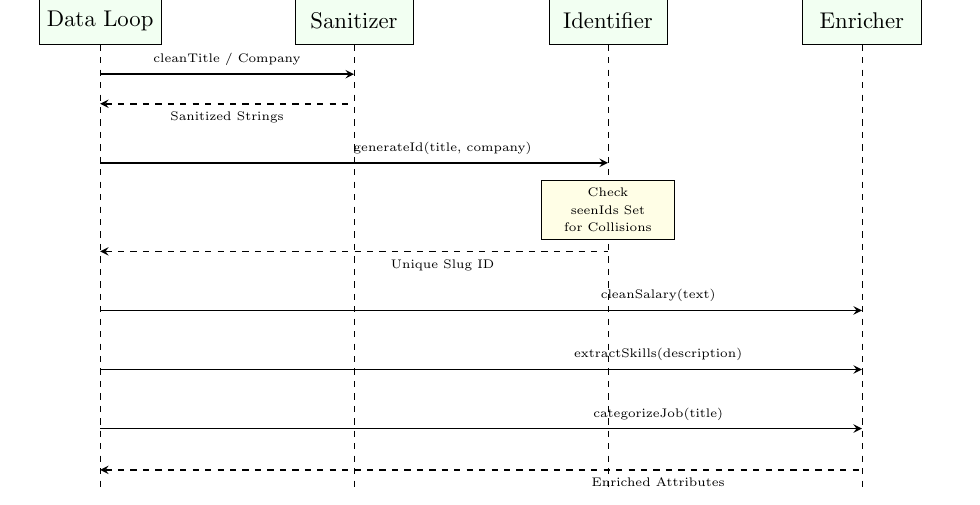
\includegraphics[width=0.7\textwidth]{figures/fig_enrichment_lifecycle}
    \caption{Sequential processing from raw ingestion to structured cache.}
\end{frame}

\begin{frame}{Hybrid Retrieval Strategy}
    \begin{columns}
        \begin{column}{0.5\textwidth}
            \textbf{Lexical (BM25):}
            \begin{itemize}
                \item Matches exact skill names and acronyms.
                \item Handles branded searches (Company names).
            \end{itemize}
            \textbf{Semantic (HNSW):}
            \begin{itemize}
                \item Captures meaning and synonyms.
                \item Overcomes the lexical gap.
            \end{itemize}
        \end{column}
        \begin{column}{0.5\textwidth}
            \centering
            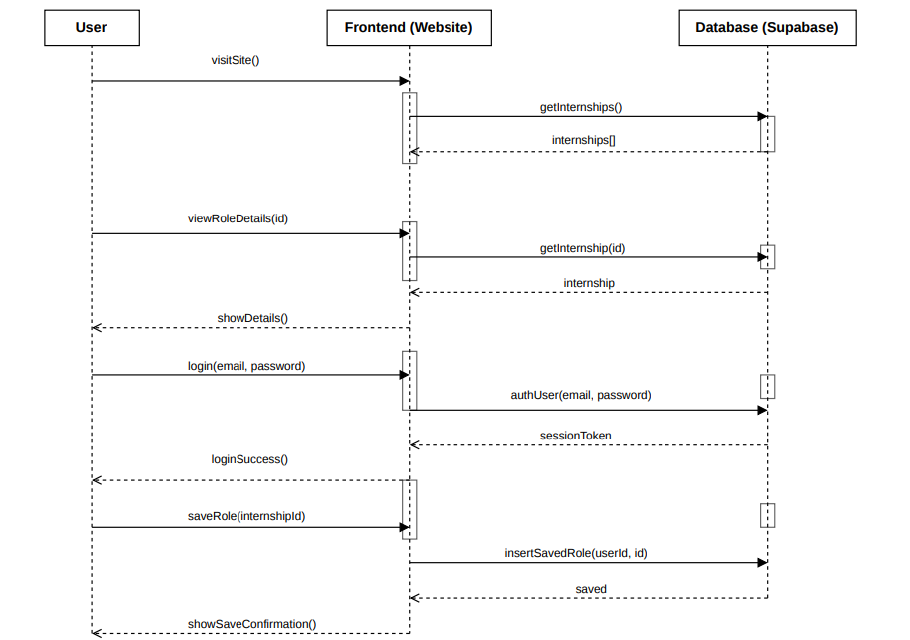
\includegraphics[width=1.1\textwidth]{figures/fig_retrieval_seq}
        \end{column}
    \end{columns}
\end{frame}

\begin{frame}{Fusion with Reciprocal Rank Fusion (RRF)}
    \begin{itemize}
        \item Combines lexical and dense retrieval outputs using rank positions.
        \item \textbf{Formula:}
            \[ \text{RRF\_score}(d) = \sum_{r \in \{\text{bm25}, \text{vector}\}} \frac{1}{k + \text{rank}_r(d)} \]
        \item \textbf{Properties:}
            \begin{itemize}
                \item \textbf{Scale-invariant:} No need to normalize disparate scores.
                \item \textbf{Robust:} Constant $k=60$ smooths outliers.
                \item \textbf{Effective:} Prioritizes consensus between retrieval models.
            \end{itemize}
    \end{itemize}
\end{frame}

% --- Evaluation ---
\section{Evaluation}

\begin{frame}{Evaluation Methodology}
    \begin{itemize}
        \item \textbf{Dataset:} 17,500 real-world internship listings.
        \item \textbf{Metrics:}
            \begin{itemize}
                \item \textbf{Retrieval Quality:} HR@10, NDCG@10.
                \item \textbf{Accuracy:} Precision/Recall for ESCO classification.
                \item \textbf{Efficiency:} p50/p99 Latency, Memory RSS.
                \item \textbf{Cost:} Comparative cost vs. pure LLM approach.
            \end{itemize}
        \item \textbf{Hardware:} Commodity Workstation (i7-13700K, 32GB RAM, No GPU).
    \end{itemize}
\end{frame}

\begin{frame}{Results Highlights}
    \begin{itemize}
        \item \textbf{Performance:} Median retrieval latency of $\sim$47 ms.
        \item \textbf{Semantic Lift:} $\sim$29\% improvement in NDCG@10 with hybrid search.
        \item \textbf{Cost Efficiency:} $>95\%$ reduction in inference cost compared to per-query LLM.
        \item \textbf{Classification:} DistilBERT achieves high F1 for standard professional domains.
    \end{itemize}
\end{frame}

% --- Conclusion ---
\section{Conclusion}

\begin{frame}{Summary and Future Work}
    \textbf{Key Takeaways:}
    \begin{itemize}
        \item Modular, tiered architecture successfully balances cost and accuracy.
        \item Lightweight models provide sufficient semantic power for the internship domain.
        \item Hybrid search significantly improves discovery relevance.
    \end{itemize}

    \textbf{Future Work:}
    \begin{itemize}
        \item Real-time stream processing for scraping ingestion.
        \item Expansion to multi-lingual listings and global taxonomies.
        \item Integration of personalized user-profile embeddings for recommendation.
    \end{itemize}
\end{frame}

\begin{frame}
    \centering
    \Huge Thank you! \\ \vspace{1cm} \large Questions?
\end{frame}

\end{document}
